\documentclass[table]{beamer}
\usepackage[utf8]{inputenc}
\usepackage[squaren]{SIunits}
\usepackage{varwidth,setspace}
\usepackage{tikz}
\usetikzlibrary{intersections,positioning,backgrounds,fit,matrix,shapes,calc,decorations.pathmorphing,decorations.text,decorations.pathreplacing}
\usetheme{default}

\newcommand*{\mimg}[2]{\begingroup
\setbox0=\hbox{\includegraphics[height=#2]{#1}}\parbox{\wd0}{\box0}\endgroup}
\newcommand*{\rmimg}[2]{\begingroup
\setbox0=\hbox{\includegraphics[angle=90,origin=c,height=#2]{#1}}\parbox{\wd0}{\box0}\endgroup}

\newcommand\independent{\protect\mathpalette{\protect\independenT}{\perp}}\def\independenT#1#2{\mathrel{\rlap{$#1#2$}\mkern2mu{#1#2}}}

\setbeamertemplate{navigation symbols}{}%remove navigation symbols
\setbeamertemplate{footline}{\hspace*{.5cm}\scriptsize{\hfill\raisebox{1mm}{\insertframenumber}\hspace*{.5cm}}}

\setlength{\tabcolsep}{0.5mm}

\title{HD imaging of the CMB with ACT}
\author{Sigurd Kirkevold Næss}
\institute{Subdepartment of astrophysics, Oxford University}
\date{February, 2015}

\begin{document}


% New overall thread
%    * Will talk about recent ACT measurements.
\begin{frame}
	\titlepage
	\vspace{-1cm}
	\begin{center}
	{\footnotesize The source code for this talk can be found at {\color[rgb]{0,0.7,0}https://github.com/amaurea/actpol-talk-2015}}
	\end{center}
\end{frame}
%    * Short CMB intro. Big bang, surface of last scattering, picture of early universe
%      everyithing simple and linear, radiation much more relevant: gravitational waves
{
\usebackgroundtemplate{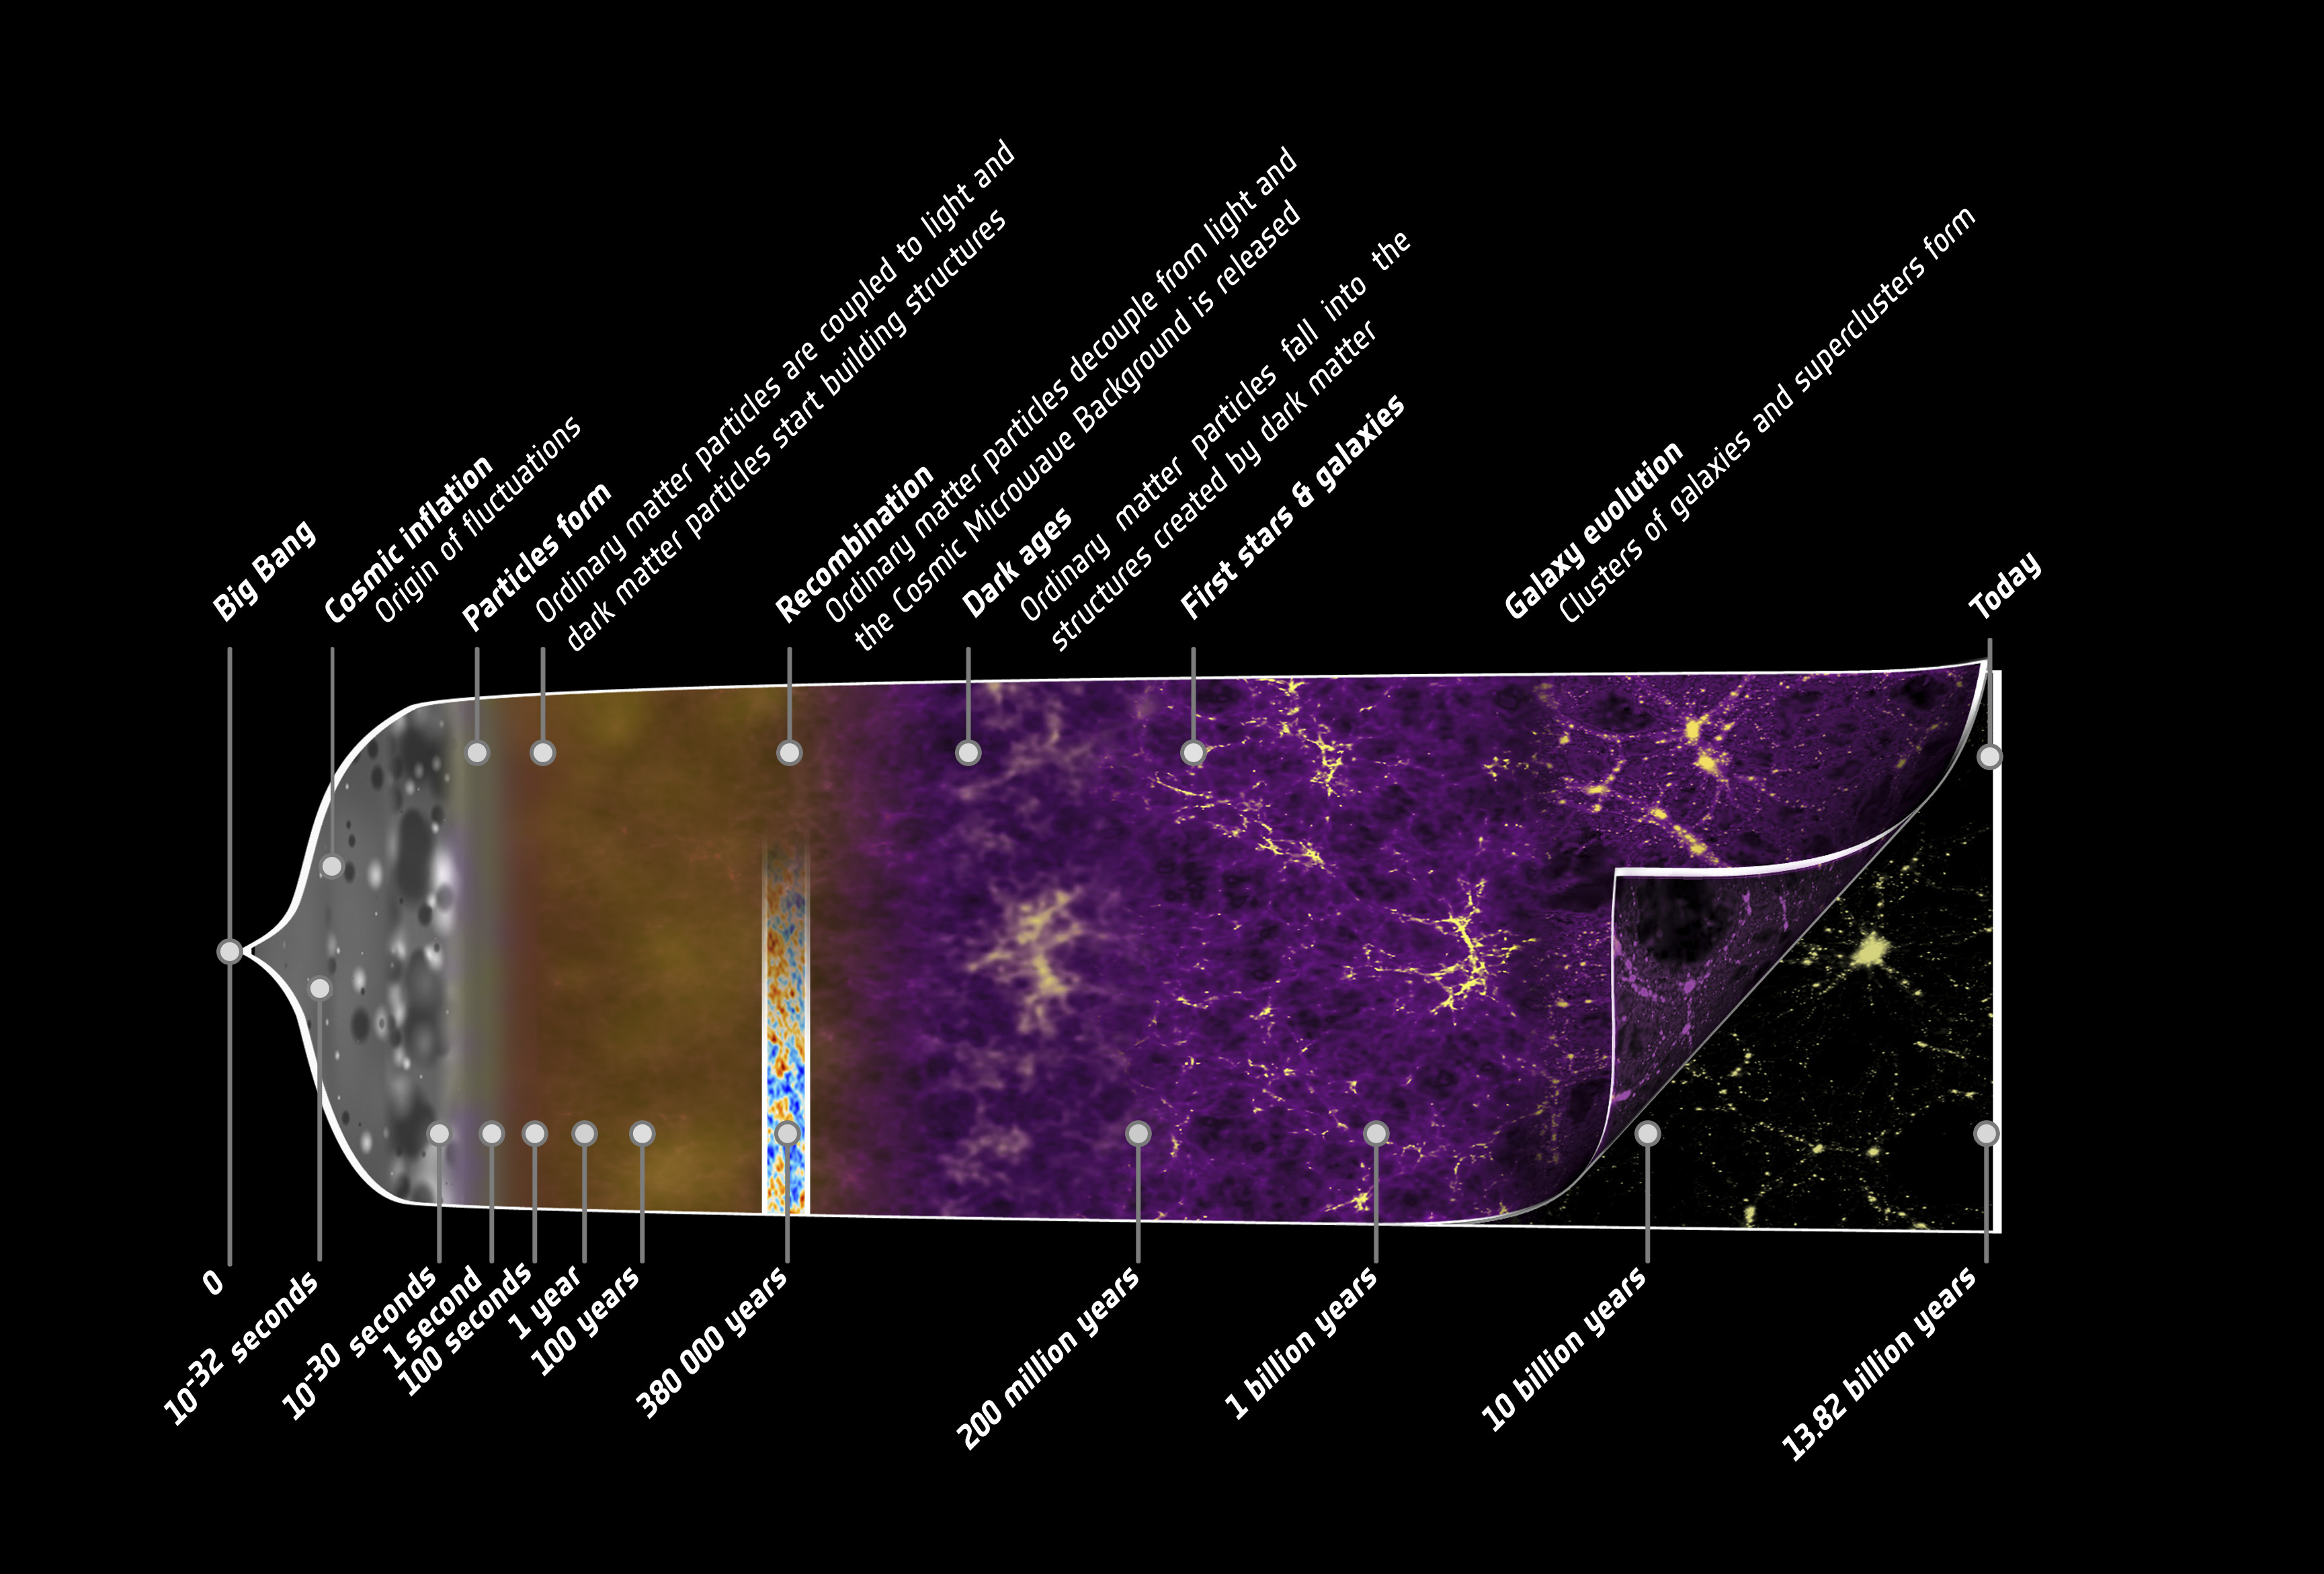
\includegraphics[width=\paperwidth,height=\paperheight]{planck_esa_history_universe.jpeg}}%
\begin{frame}[fragile]{The mandatory slide}
	\centering
	\begin{tikzpicture}[remember picture,overlay]
		\node[rotate=90,red,thick] at (0.2,-1.3) {\huge ???};
		\node[red,thick] at (1.1,-1.3) {\huge ?};
		\node[red,thick] at (2.5,-1.3) {\huge Simple};
		\node[red,thick] at (7.3,-1.3) {\huge Messy};
		\node[white] at (5,-4.5) {\footnotesize{Credit: Planck}};
	\end{tikzpicture}
\end{frame}
}

\begin{frame}{The Cosmic Microwave background}
	\begin{tikzpicture}
		\node[text width=6cm] at (0,0) {
			\begin{itemize}
				\item<1-> Almost isotropic
				\item<2-> Fluctuations of 1 part in 10\,000
				\item<3-> Black-body, 3000K $\rightarrow$ 2.73K. Same information at every frequency.
				\item<4-> E-mode polarization: 1 part in $10^{-5}$
				\item<5-> B-mode polarization: ?
			\end{itemize}
		};
		\uncover<1>{\node at (6,-0.5) {
\includegraphics[width=5cm]{mtot.png}};}
		\uncover<2>{\node at (6,-0.5) {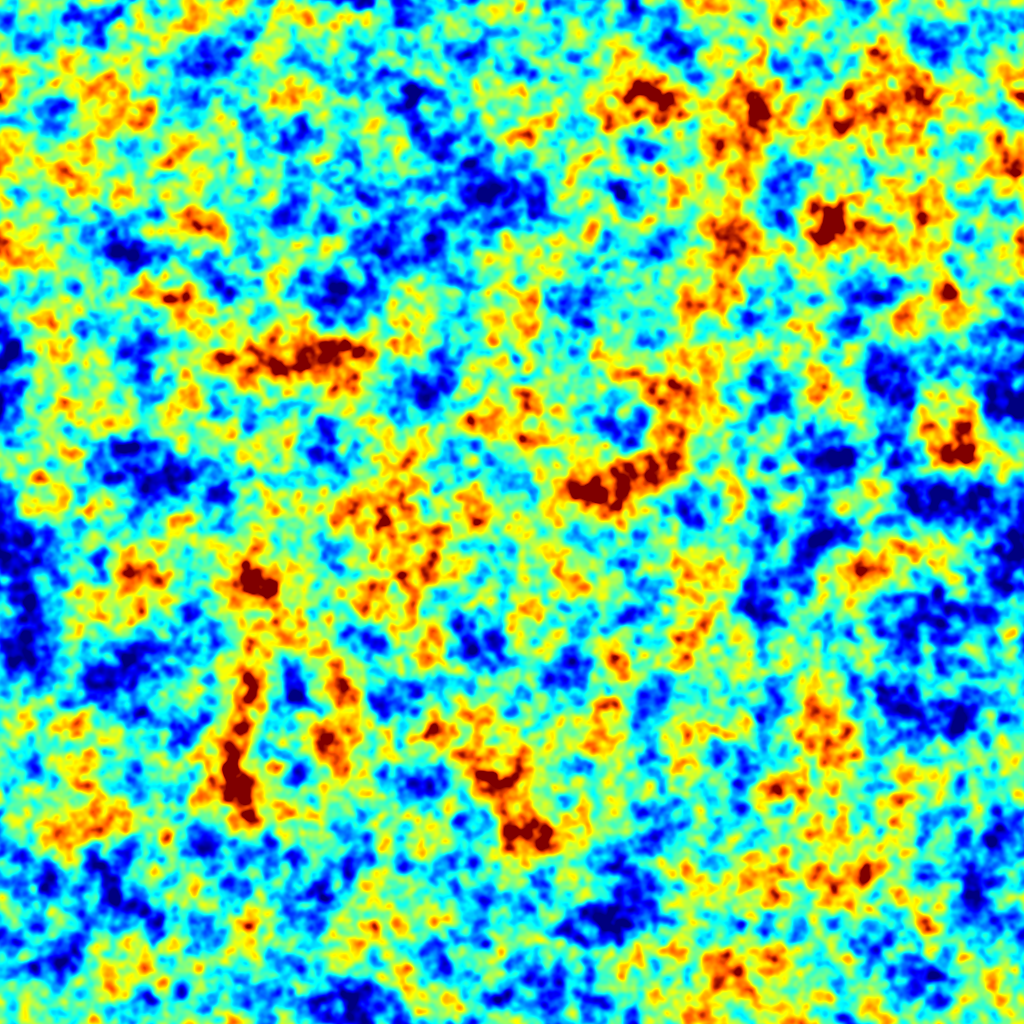
\includegraphics[width=5cm]{mdelta.png}};}
		\uncover<3>{\node at (6,-0.5) {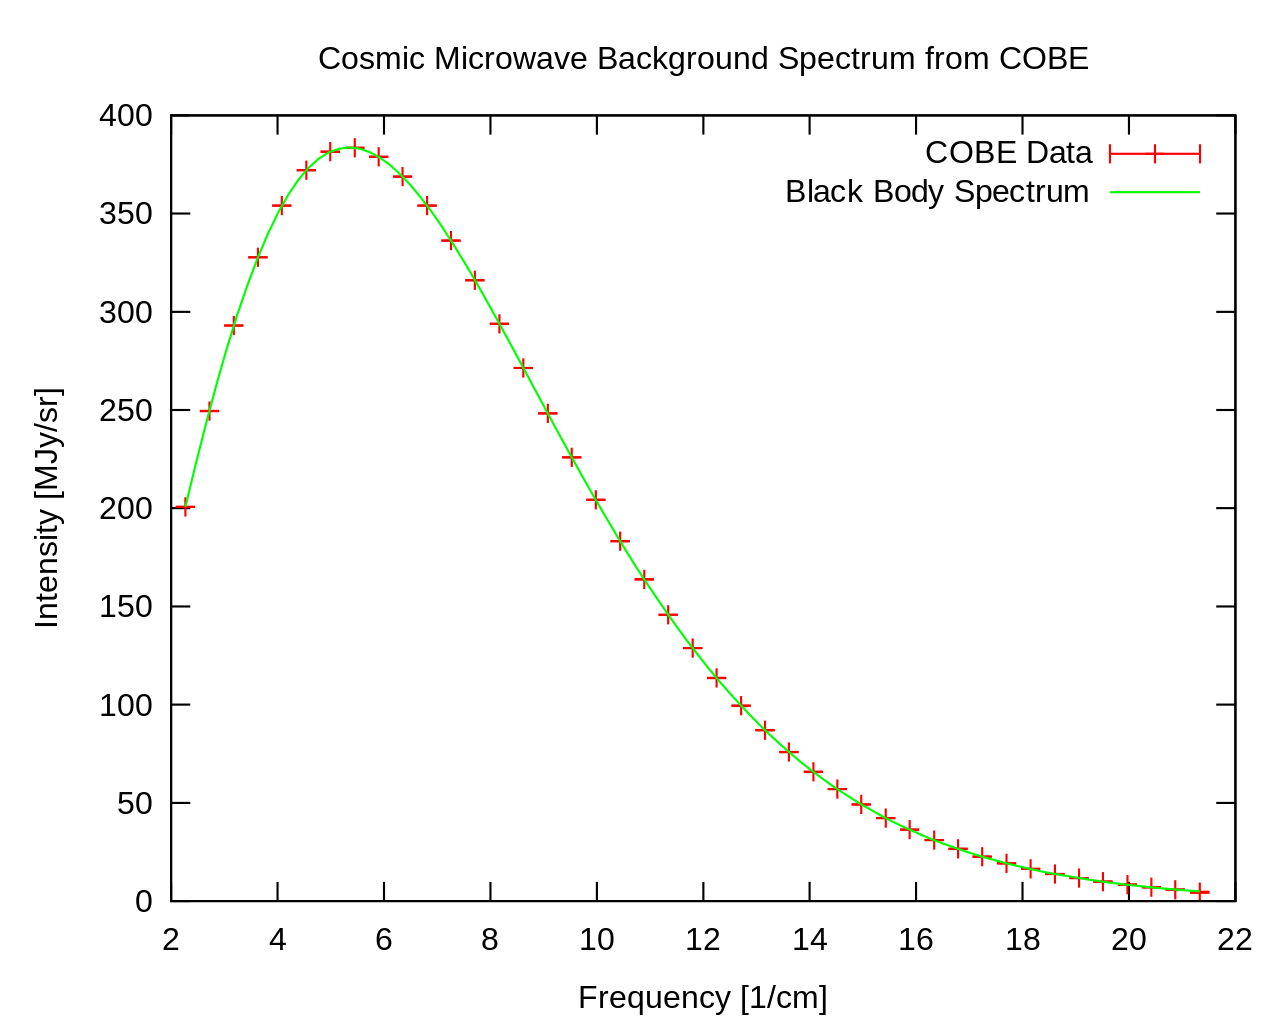
\includegraphics[width=6cm]{cobe_firas_blackbody.png}};}
		\uncover<4>{\node at (6,-0.0) {
\includegraphics[width=2cm]{E_pattern_small}};}
		\uncover<5>{\node at (6,-0.0) {
\includegraphics[width=2cm]{B_pattern_small}};}
	\end{tikzpicture}
\end{frame}

%\begin{frame}{What's so great about the CMB anyway?}
%\end{frame}
%    * More detailed about what it looks like? T, E and B generation mechanisms,
%      thompson scattering, movement perp to density countours -> E.

% 12 * But light has to travel for 13.8 billion years to tell us about all that.
%      Preilous journey. What happens to T,E and B on the way.
%    * And as it enters the telescope
\begin{frame}{From pristine CMB to dirty data}
	\begin{center}
		\large%
		\only<1>{At the surface of last scattering}%
		\only<2>{Lensing by large-scale structure}%
		\only<3>{Dusty galaxies, radio sources, SZ clusters}%
		\only<4>{Faraday rotation}%
		\only<5>{Galctic dust, synchrotron, etc}%
		\only<6>{Atmospheric emission}%
		\only<7>{Absolute polarization offset ($1^\circ$ example)}%
		\only<8>{Telescope optics (w. sidelobe)}%
		\only<9>{Detector noise}%
		\only<10>{Glitches}%
		\uncover<1-0>{()}% Dummy to keep line height constant
	\end{center}
	\begin{tikzpicture}[thick,red,decoration={snake, amplitude=1mm,segment length = 5mm}]
		\node at (0.0,0) (A) {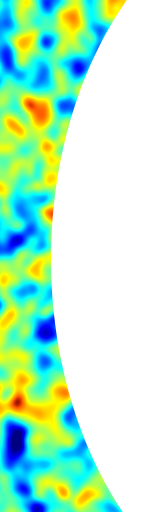
\includegraphics[height=1cm]{sls.png}};
		\node at (2.5,0) (B) {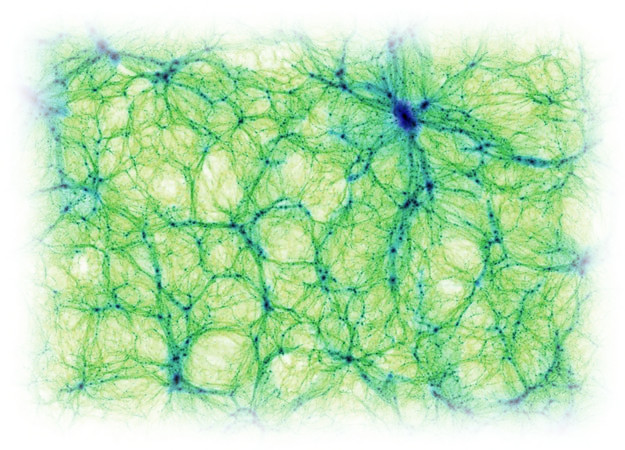
\includegraphics[height=1.5cm]{lss.jpeg}};
		\node at (5.0,0) (C) {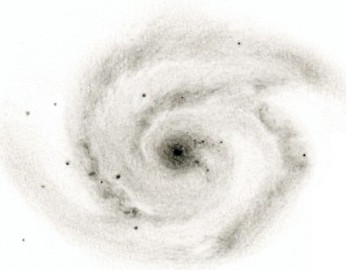
\includegraphics[height=1cm]{galaxy.jpeg}};
		\node at (7.5,0) (D) {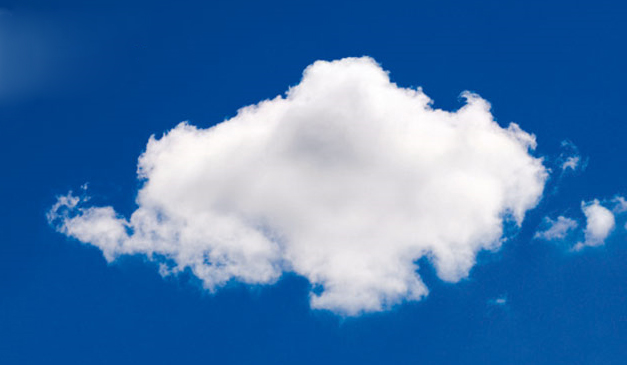
\includegraphics[height=1cm]{cloud.jpg}};
		\node at (10.0,0) (E) {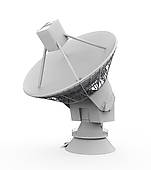
\includegraphics[height=1cm]{telescope.jpg}};
		\only<1>{\draw [decorate] (0,0) -- (0.5,0);}%
		\only<2-3>{\draw [decorate] (0,0) -- (2.5,0);}%
		\only<4-5>{\draw [decorate] (0,0) -- (5.0,0);}%
		\only<6>{\draw [decorate] (0,0) -- (7.5,0);}%
		\only<7-10>{\draw [decorate] (0,0) -- (10.0,0);}%
	\end{tikzpicture}
	\hspace*{-5mm}\begin{tabular}{ccc}
		T&E&B\\
	\only<1>{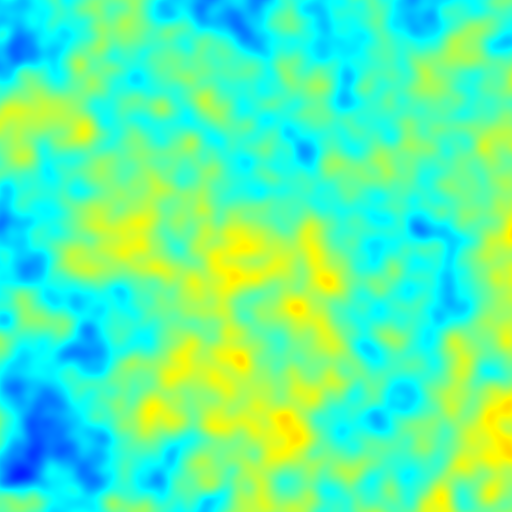
\includegraphics[width=0.35\textwidth]{contaminants/01_cmb_teb_0.png}}%
	\only<2>{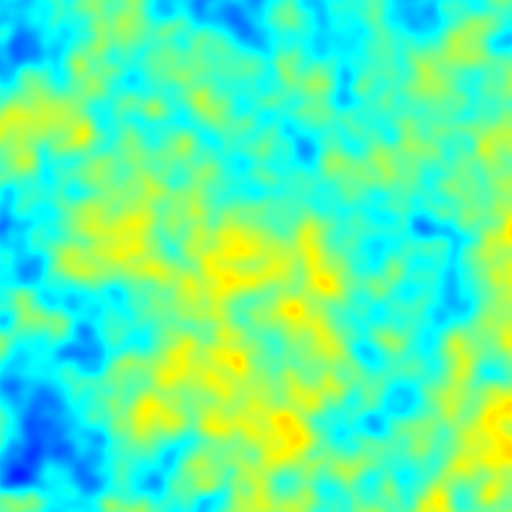
\includegraphics[width=0.35\textwidth]{contaminants/02_lens_teb_0.png}}%
	\only<3>{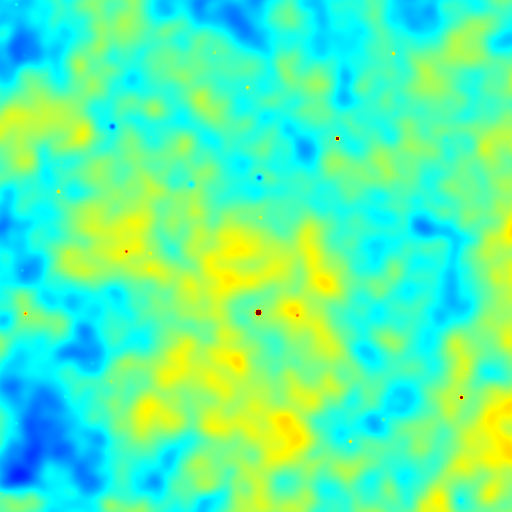
\includegraphics[width=0.35\textwidth]{contaminants/04_sz_teb_0.png}}%
	\only<4>{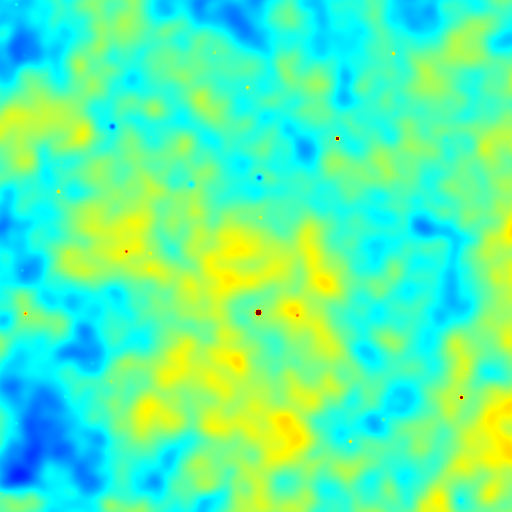
\includegraphics[width=0.35\textwidth]{contaminants/05_faraday_teb_0.png}}%
	\only<5>{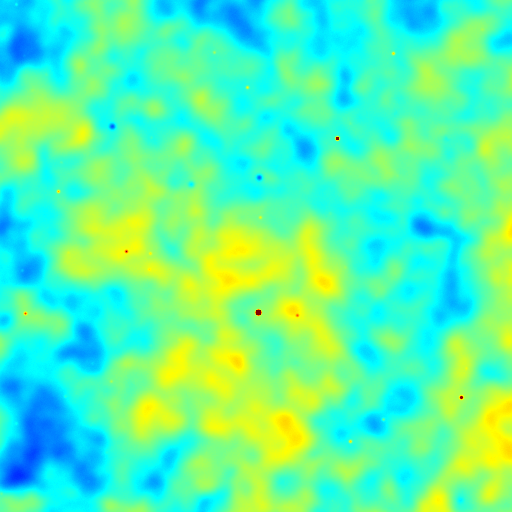
\includegraphics[width=0.35\textwidth]{contaminants/06_dust_teb_0.png}}%
	\only<6>{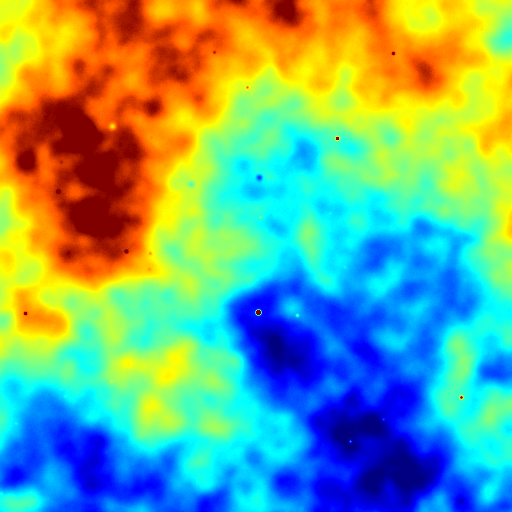
\includegraphics[width=0.35\textwidth]{contaminants/07_atm_teb_0.png}}%
	\only<7>{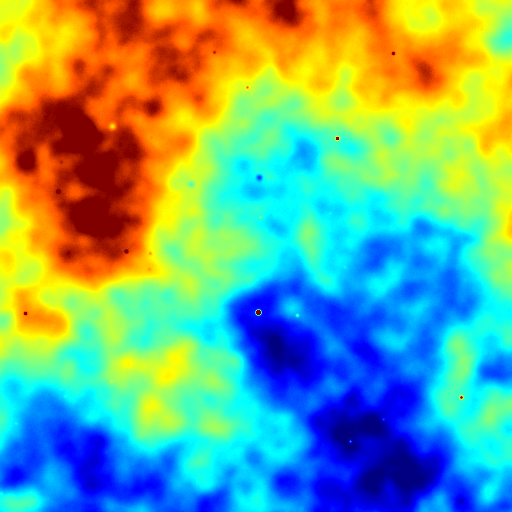
\includegraphics[width=0.35\textwidth]{contaminants/08_polerr_teb_0.png}}%
	\only<8>{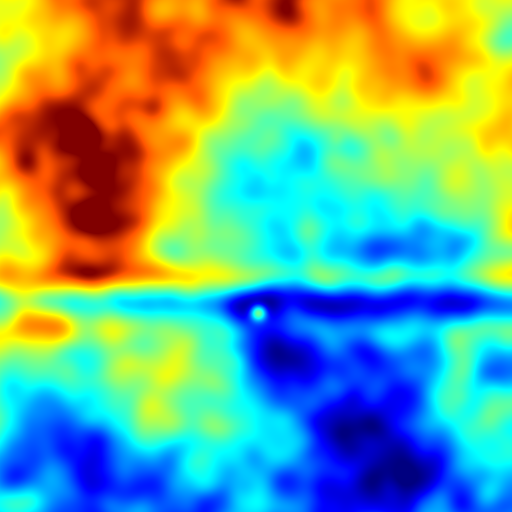
\includegraphics[width=0.35\textwidth]{contaminants/10_beam_teb_0.png}}%
	\only<9>{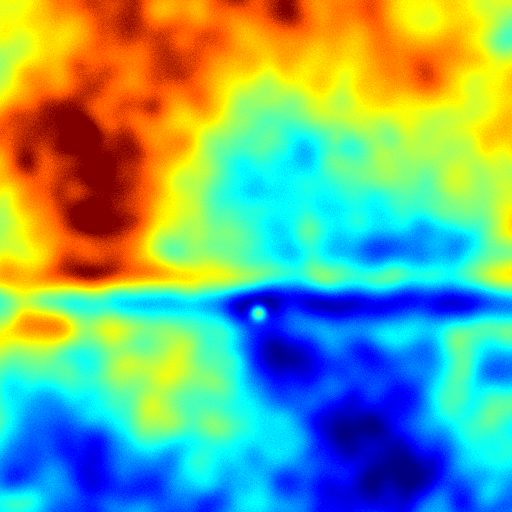
\includegraphics[width=0.35\textwidth]{contaminants/11_noise_teb_0.png}}%
	\only<10>{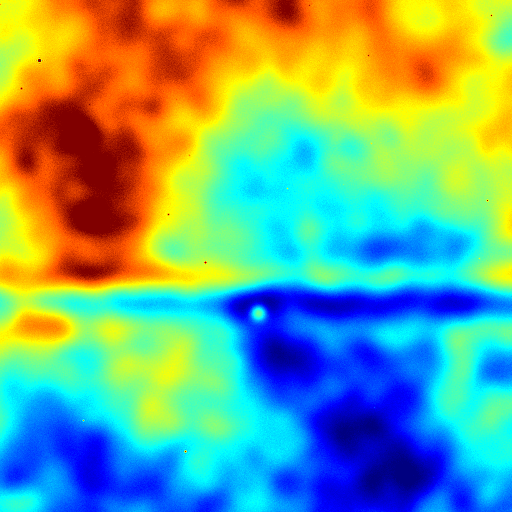
\includegraphics[width=0.35\textwidth]{contaminants/12_glitch_teb_0.png}}%
	&
	\only<1>{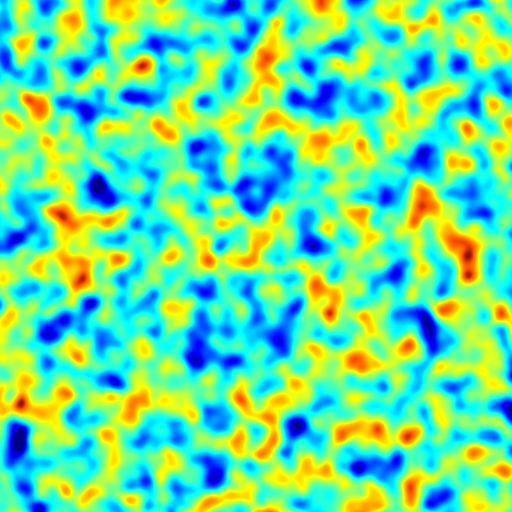
\includegraphics[width=0.35\textwidth]{contaminants/01_cmb_teb_1.png}}%
	\only<2>{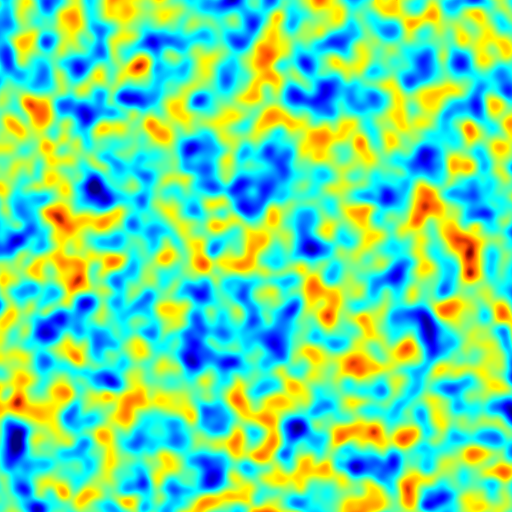
\includegraphics[width=0.35\textwidth]{contaminants/02_lens_teb_1.png}}%
	\only<3>{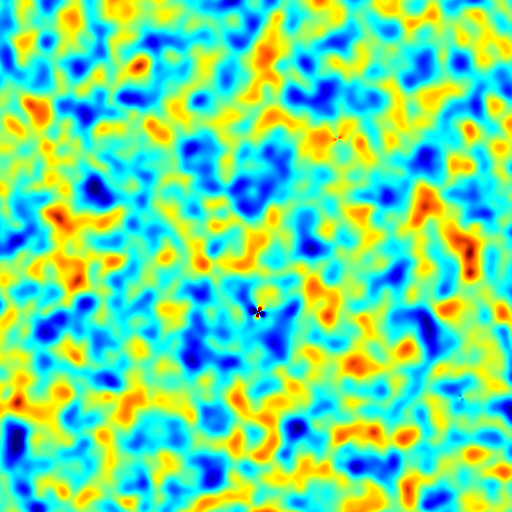
\includegraphics[width=0.35\textwidth]{contaminants/04_sz_teb_1.png}}%
	\only<4>{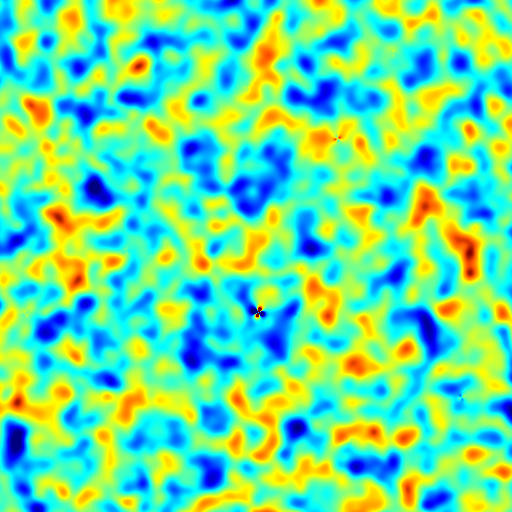
\includegraphics[width=0.35\textwidth]{contaminants/05_faraday_teb_1.png}}%
	\only<5>{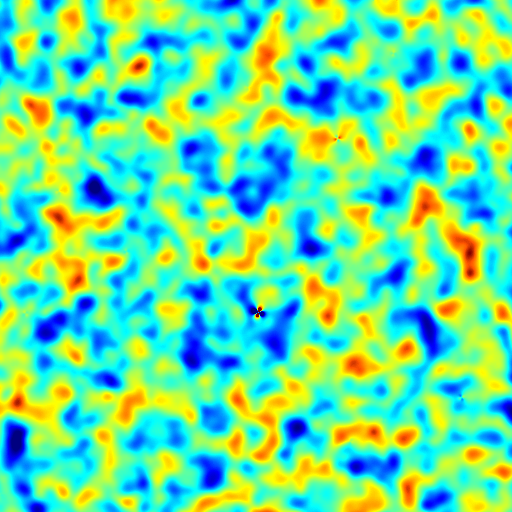
\includegraphics[width=0.35\textwidth]{contaminants/06_dust_teb_1.png}}%
	\only<6>{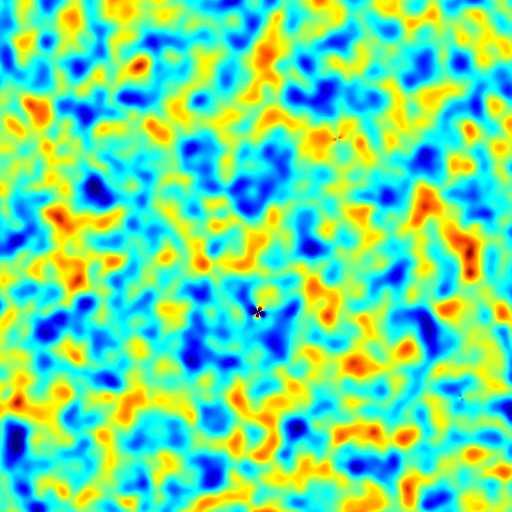
\includegraphics[width=0.35\textwidth]{contaminants/07_atm_teb_1.png}}%
	\only<7>{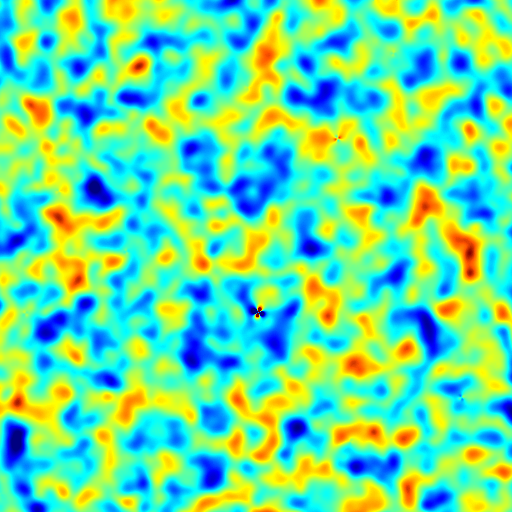
\includegraphics[width=0.35\textwidth]{contaminants/08_polerr_teb_1.png}}%
	\only<8>{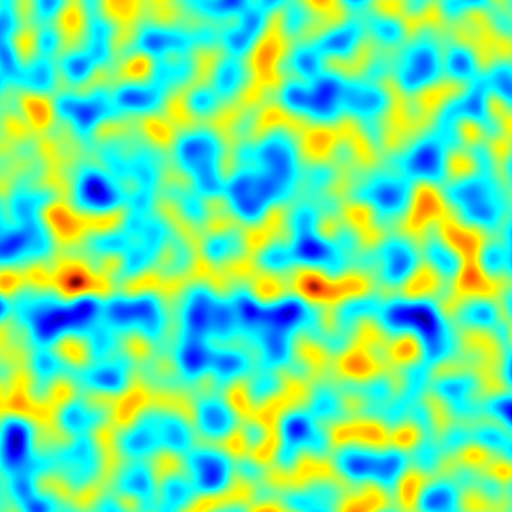
\includegraphics[width=0.35\textwidth]{contaminants/10_beam_teb_1.png}}%
	\only<9>{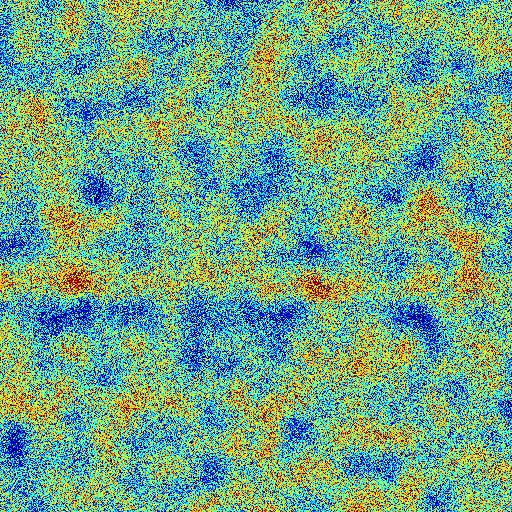
\includegraphics[width=0.35\textwidth]{contaminants/11_noise_teb_1.png}}%
	\only<10>{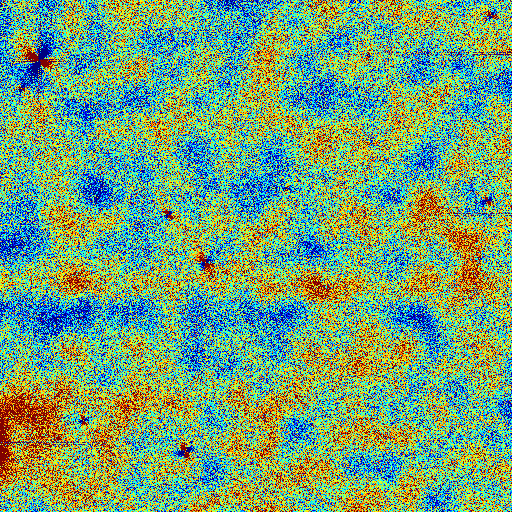
\includegraphics[width=0.35\textwidth]{contaminants/12_glitch_teb_1.png}}%
	&
	\only<1>{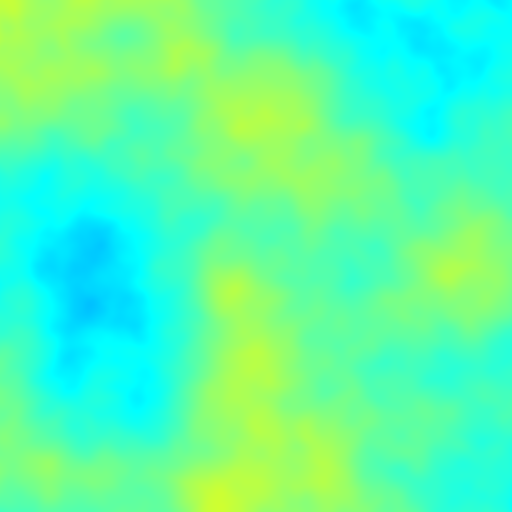
\includegraphics[width=0.35\textwidth]{contaminants/01_cmb_teb_2.png}}%
	\only<2>{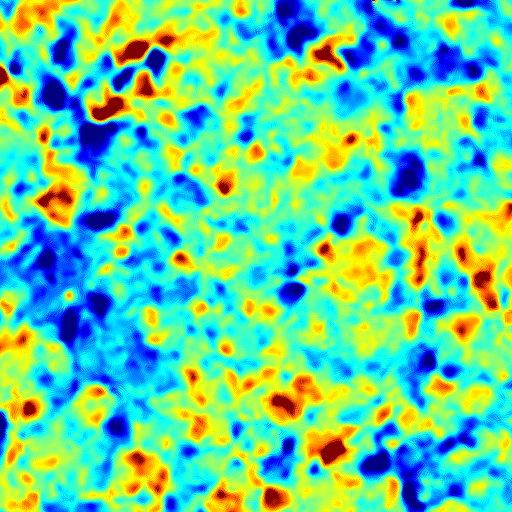
\includegraphics[width=0.35\textwidth]{contaminants/02_lens_teb_2.png}}%
	\only<3>{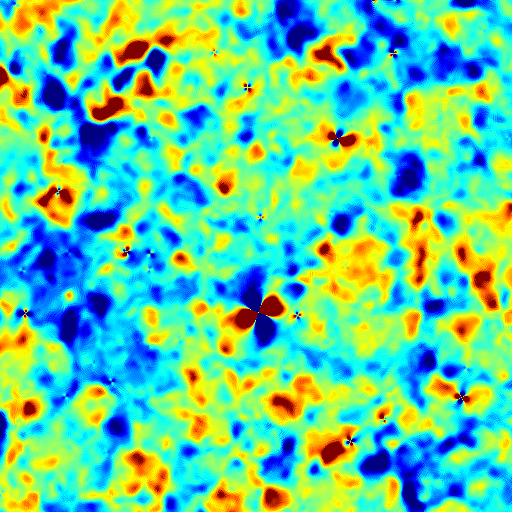
\includegraphics[width=0.35\textwidth]{contaminants/04_sz_teb_2.png}}%
	\only<4>{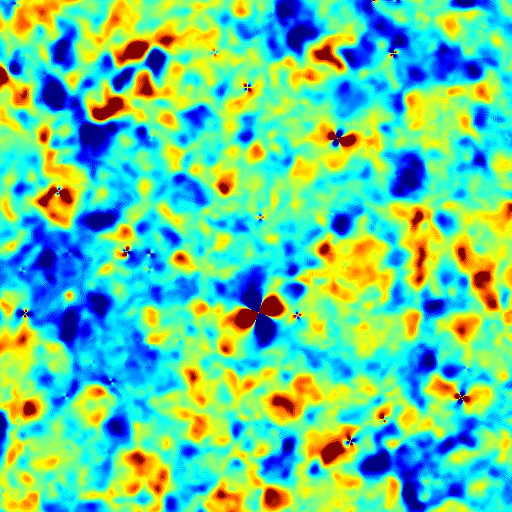
\includegraphics[width=0.35\textwidth]{contaminants/05_faraday_teb_2.png}}%
	\only<5>{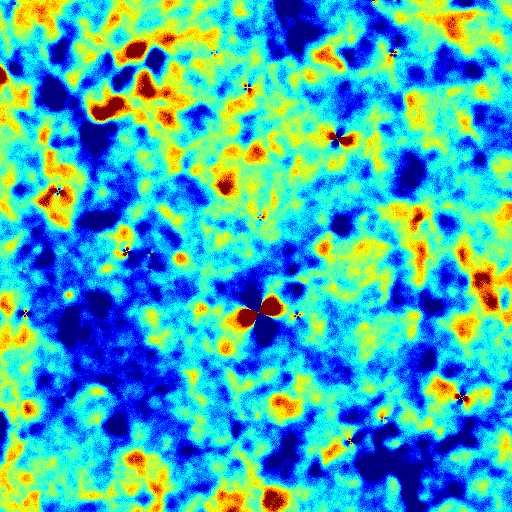
\includegraphics[width=0.35\textwidth]{contaminants/06_dust_teb_2.png}}%
	\only<6>{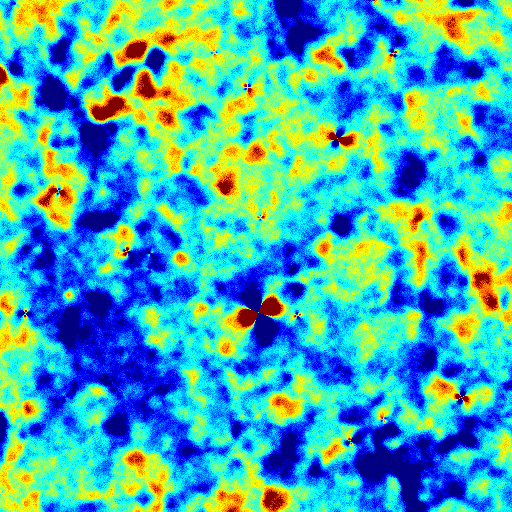
\includegraphics[width=0.35\textwidth]{contaminants/07_atm_teb_2.png}}%
	\only<7>{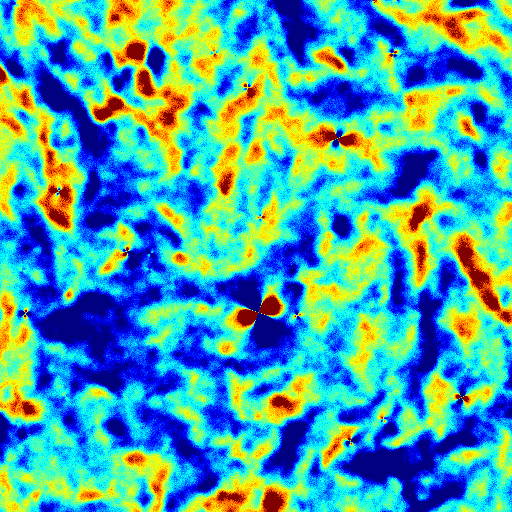
\includegraphics[width=0.35\textwidth]{contaminants/08_polerr_teb_2.png}}%
	\only<8>{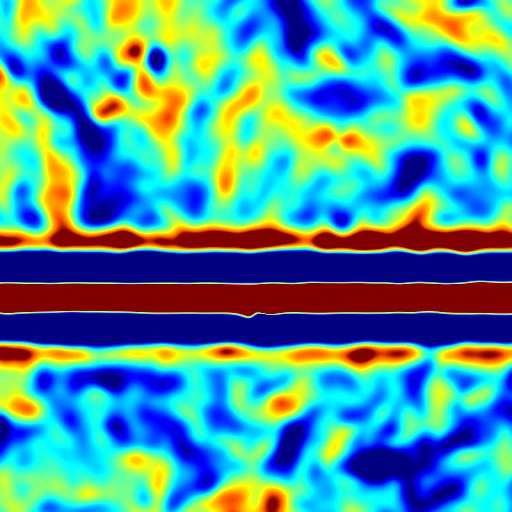
\includegraphics[width=0.35\textwidth]{contaminants/10_beam_teb_2.png}}%
	\only<9>{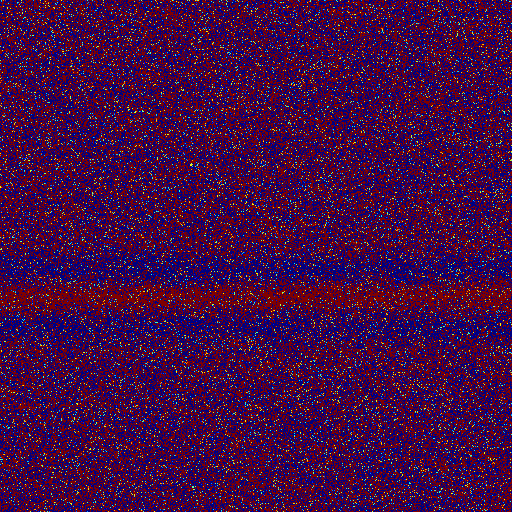
\includegraphics[width=0.35\textwidth]{contaminants/11_noise_teb_2.png}}%
	\only<10>{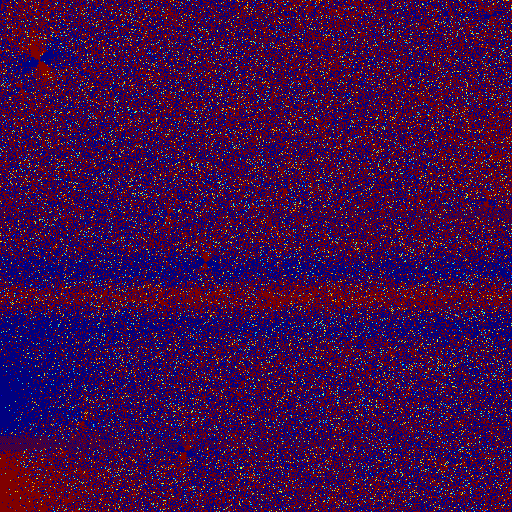
\includegraphics[width=0.35\textwidth]{contaminants/12_glitch_teb_2.png}}%
	\\
	{\footnotesize $-500\mu$K\enskip
\includegraphics[width=12mm,height=2mm]{colorbar.png}\enskip$500\mu$K} &
	{\footnotesize $-20\mu$K\enskip
\includegraphics[width=12mm,height=2mm]{colorbar.png}\enskip$20\mu$K} &
	{\footnotesize $-1\mu$K\enskip
\includegraphics[width=12mm,height=2mm]{colorbar.png}\enskip$1\mu$K}
\end{tabular}\hspace*{-5mm}
\end{frame}
%    * What telescope measures etc.
\begin{frame}{What the telescope actually observes}
	\begin{tikzpicture}[bad/.style={line width=3pt,red}]
		\node at (0,0) {\begin{tabular}{ccc}
				T & E & B \\
				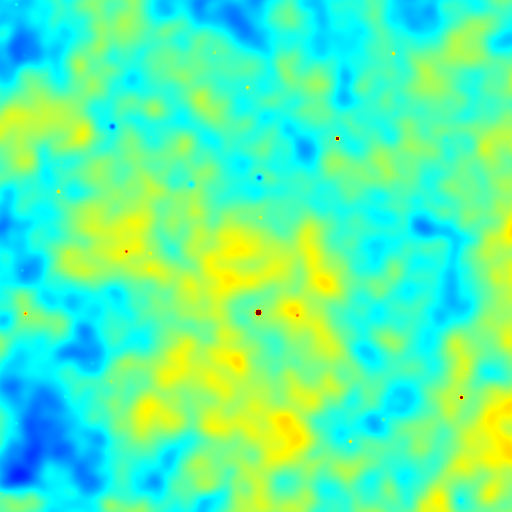
\includegraphics[width=0.30\textwidth]{contaminants/04_sz_teb_0.png} &
				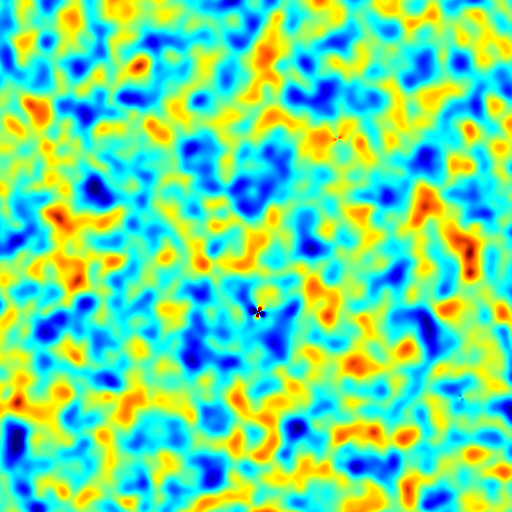
\includegraphics[width=0.30\textwidth]{contaminants/04_sz_teb_1.png} &
				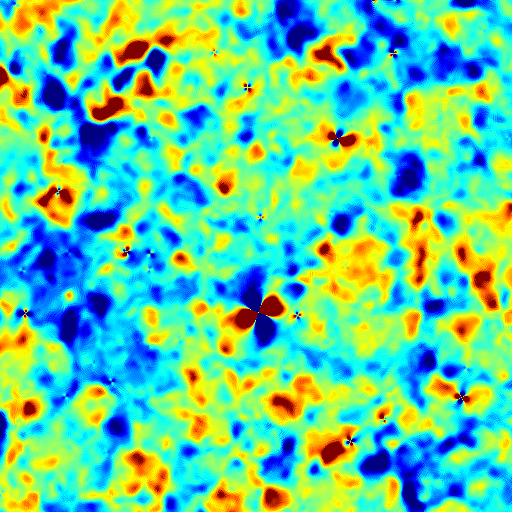
\includegraphics[width=0.30\textwidth]{contaminants/04_sz_teb_2.png}
		\end{tabular}};
		\uncover<2->{%
		\draw[bad] (-5, 1.5) -- (5,-1.8);
		\draw[bad] (-5,-1.8) -- (5, 1.5);}
		\node at (0,-4) {\begin{tabular}{ccc}
				\only<3-4>{T+pol}\only<5->{T} & \uncover<5->{Q} & \uncover<5->{U} \\
				\only<3-4>{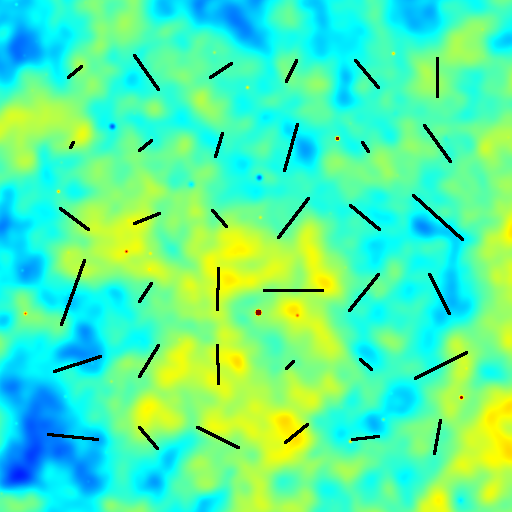
\includegraphics[width=0.30\textwidth]{contaminants/t_polvec.png}}%
				\only<5->{\includegraphics[width=0.30\textwidth]{contaminants/04_sz_tqu_0.png}} &
				\uncover<5->{\includegraphics[width=0.30\textwidth]{contaminants/04_sz_tqu_1.png}} &
				\uncover<5->{\includegraphics[width=0.30\textwidth]{contaminants/04_sz_tqu_2.png}}
		\end{tabular}};
		\uncover<4>{\node at (1.5,-4) {\includegraphics[height=3cm]{qudef_healpix.pdf}};}
	\end{tikzpicture}
\end{frame}

\begin{frame}{E,B and Q, U}
	\begin{center}
		\only<1>{E and B result from quadrupole-convolutions of Q and U}%
		%\only<2>{Reverse also holds}%

	\scalebox{1.7}{
		\begin{minipage}{5cm}
			\begin{align*}
				\only<1>{%
				E =& \rmimg{contaminants/queb_0.png}{1cm} \otimes Q + \mimg{contaminants/queb_2.png}{1cm} \otimes U \\
				B =& \mimg{contaminants/queb_1.png}{1cm} \otimes Q + \rmimg{contaminants/queb_3.png}{1cm} \otimes U}%
				%\only<2>{%
				%Q =& \rmimg{contaminants/ebqu_0.png}{1cm} \otimes E + \mimg{contaminants/ebqu_2.png}{1cm} \otimes B \\
				%U =& \mimg{contaminants/ebqu_1.png}{1cm} \otimes E + \rmimg{contaminants/ebqu_3.png}{1cm} \otimes B}%
			\end{align*}
		\end{minipage}}
	\end{center}
\end{frame}

\begin{frame}{Actually only observe linear combinations}
	\begin{center}
	\begin{tabular}{c}
		\only<1>{Detector 1: T+Q}%
		\only<2>{Detector 2: T+U}%
		\only<3>{Detector 3: T-Q}%
		\only<4>{Detector 4: T-U}%
		\\
		\only<1>{\includegraphics[height=7cm]{contaminants/tqu_lincombs_0.png}}%
		\only<2>{\includegraphics[height=7cm]{contaminants/tqu_lincombs_1.png}}%
		\only<3>{\includegraphics[height=7cm]{contaminants/tqu_lincombs_2.png}}%
		\only<4>{\includegraphics[height=7cm]{contaminants/tqu_lincombs_3.png}}%
	\end{tabular}
\end{center}
\end{frame}

\begin{frame}{Not like a digital camera}
	\begin{tikzpicture}[bad/.style={line width=8pt,red},scan/.style={thick,red}]
		\node at (0,0) (A) {\includegraphics[height=3cm]{contaminants/06_dust_teb_0.png}};
		\uncover<2->{%
		\node at (1.5,-1) (B) {\includegraphics[height=3cm]{camera.png}};}
		\uncover<3->{%
		\draw[bad] (-1.1,-2.1) -- ( 2.6, 1.6);
		\draw[bad] (-1.1, 1.6) -- ( 2.6,-2.1);}
		\uncover<4->{%
		\node at (6,0) (C) {\includegraphics[height=3cm]{contaminants/06_dust_teb_0.png}};}
		\uncover<5->{%
		\draw[scan] (5, 1.0) -- (7, 0.9);}
		\uncover<6->{%
		\draw[scan] (7, 0.9) -- (5, 0.8);}
		\uncover<7->{%
		\draw[scan] (5, 0.8) -- (7, 0.7);}
		\uncover<8->{%
		\draw[scan] (7, 0.7) -- (5, 0.6);}
		\uncover<9->{%
		\draw[scan] (5, 0.6) -- (7, 0.5);}
		\uncover<10->{%
		\draw[scan] (7, 0.5) -- (5, 0.4);}
		\uncover<11->{%
		\draw[scan] (5, 0.4) -- (7, 0.3);
		\draw[scan] (7, 0.3) -- (5, 0.2);
		\draw[scan] (5, 0.2) -- (7, 0.1);
		\draw[scan] (7, 0.1) -- (5, 0.0);
		\draw[scan] (5, 0.0) -- (7,-0.1);
		\draw[scan] (7,-0.1) -- (5,-0.2);
		\draw[scan] (5,-0.2) -- (7,-0.3);
		\draw[scan] (7,-0.3) -- (5,-0.4);
		\draw[scan] (5,-0.4) -- (7,-0.5);
		\draw[scan] (7,-0.5) -- (5,-0.6);
		\draw[scan] (5,-0.6) -- (7,-0.7);
		\draw[scan] (7,-0.7) -- (5,-0.8);
		\draw[scan] (5,-0.8) -- (7,-0.9);
		\draw[scan] (7,-0.9) -- (5,-1.0);
	\draw[scan] (5,-1.0) -- (7,-1.1);}
		\uncover<4->{
		\node at (7.5,-1) (D) {\includegraphics[height=3cm]{telescope2.png}};}
		\uncover<5->{%
		\draw[thick,red,->,rounded corners=1mm] (7.5,-2.4) -- (7.5,-2.6) -- (-0.5,-2.6) -- (-0.5,-2.9);
		\node at (-0.5,-3.00) {\includegraphics[height=0.7mm,width=1.5cm]{contaminants/scanrow100.png}};}
		\uncover<6->{%
		\node at ( 1.0,-3.00) {\includegraphics[height=0.7mm,width=1.5cm]{contaminants/scanrow116.png}};}
		\uncover<7->{%
		\node at ( 2.5,-3.00) {\includegraphics[height=0.7mm,width=1.5cm]{contaminants/scanrow132.png}};}
		\uncover<8->{%
		\node at ( 4.0,-3.00) {\includegraphics[height=0.7mm,width=1.5cm]{contaminants/scanrow148.png}};}
		\uncover<9->{%
		\node at ( 5.5,-3.00) {\includegraphics[height=0.7mm,width=1.5cm]{contaminants/scanrow164.png}};}
		\uncover<10->{%
		\node at ( 7.0,-3.00) {\includegraphics[height=0.7mm,width=1.5cm]{contaminants/scanrow180.png}};}
		\uncover<11->{
		\node at (-0.5,-3.15) {\includegraphics[height=0.7mm,width=1.5cm]{contaminants/scanrow196.png}};
		\node at ( 1.0,-3.15) {\includegraphics[height=0.7mm,width=1.5cm]{contaminants/scanrow212.png}};
		\node at ( 2.5,-3.15) {\includegraphics[height=0.7mm,width=1.5cm]{contaminants/scanrow228.png}};
		\node at ( 4.0,-3.15) {\includegraphics[height=0.7mm,width=1.5cm]{contaminants/scanrow244.png}};
		\node at ( 5.5,-3.15) {\includegraphics[height=0.7mm,width=1.5cm]{contaminants/scanrow260.png}};
		\node at ( 7.0,-3.15) {\includegraphics[height=0.7mm,width=1.5cm]{contaminants/scanrow276.png}};
		\node at (-0.5,-3.30) {\includegraphics[height=0.7mm,width=1.5cm]{contaminants/scanrow292.png}};
		\node at ( 1.0,-3.30) {\includegraphics[height=0.7mm,width=1.5cm]{contaminants/scanrow308.png}};
		\node at ( 2.5,-3.30) {\includegraphics[height=0.7mm,width=1.5cm]{contaminants/scanrow324.png}};
		\node at ( 4.0,-3.30) {\includegraphics[height=0.7mm,width=1.5cm]{contaminants/scanrow340.png}};
		\node at ( 5.5,-3.30) {\includegraphics[height=0.7mm,width=1.5cm]{contaminants/scanrow356.png}};
		\node at ( 7.0,-3.30) {\includegraphics[height=0.7mm,width=1.5cm]{contaminants/scanrow372.png}};
		\node at (-0.5,-3.45) {\includegraphics[height=0.7mm,width=1.5cm]{contaminants/scanrow388.png}};}
	\end{tikzpicture}
	\begin{center}
		\uncover<12->{\large Time-ordered data (TOD)}
	\end{center}
\end{frame}
%    * TOD
\begin{frame}{Example TOD}
	\begin{center}
		\vspace{-1.5cm}
		\begin{tikzpicture}
			\node at (0,0) {\includegraphics[width=\textwidth]{example_tod.png}};
			\uncover<7->{%
			\draw (-1.2, 0.4) ellipse (4mm and 7mm);
			\draw (2.70,0.7) ellipse (4mm and 12mm);}
		\end{tikzpicture}
		\uncover<2->{%
		\begin{block}{Ingredients}
			\begin{columns}
				\begin{column}{5cm}
					\begin{itemize}
						\item<2-> 90\% atmospheric noise
						\item<3-> 10\% instrumental noise
						\item<4-> 0.4\% T-modes
					\end{itemize}
				\end{column}
				\begin{column}{5cm}
					\begin{itemize}
						\item<5-> 0.002\% E-modes
						\item<6-> 0.0002\% B-modes
						\item<7-> and a few glitches
					\end{itemize}
				\end{column}
			\end{columns}
		\end{block}}
	\end{center}
\end{frame}
%    * Image reconstruction
\begin{frame}{Recovering the sky}
	Can model TOD as linear combination of CMB and noise:
	\[ d = {\color{green}P}{\color{blue}s} + {\color{red}n} \]
	with TOD $d$,
	scan pattern + telescope response {\color{green} $P$},
	cmb map {\color{blue} $s$}, gaussian noise {\color{red} $n$} with cov {\color{red}$N$}.
	Then
	\[ {\color{blue}s} = ({\color{green}P}^T{\color{red}N}^{-1}{\color{green}P})^{-1}{\color{green}P}^T{\color{red}N}^{-1}d \]
	is an optimal estimator.
\end{frame}
%    * Beat down noise (white)
\begin{frame}{Throw samples at it to beat down noise}
	\begin{center}
	\hspace*{-1.4cm}\begin{tabular}{ccc}
		T & Q & U \\
		\only<1>{%
		\includegraphics[height=4cm]{maps/scansims/scansims_000_0.png} &
		\includegraphics[height=4cm]{maps/scansims/scansims_000_1.png} &
		\includegraphics[height=4cm]{maps/scansims/scansims_000_2.png}}%
		\only<2>{%
		\includegraphics[height=4cm]{maps/scansims/scansims_001_0.png} &
		\includegraphics[height=4cm]{maps/scansims/scansims_001_1.png} &
		\includegraphics[height=4cm]{maps/scansims/scansims_001_2.png}}%
		\only<3>{%
		\includegraphics[height=4cm]{maps/scansims/scansims_002_0.png} &
		\includegraphics[height=4cm]{maps/scansims/scansims_002_1.png} &
		\includegraphics[height=4cm]{maps/scansims/scansims_002_2.png}}%
		\only<4>{%
		\includegraphics[height=4cm]{maps/scansims/scansims_003_0.png} &
		\includegraphics[height=4cm]{maps/scansims/scansims_003_1.png} &
		\includegraphics[height=4cm]{maps/scansims/scansims_003_2.png}}%
		\only<5>{%
		\includegraphics[height=4cm]{maps/scansims/scansims_004_0.png} &
		\includegraphics[height=4cm]{maps/scansims/scansims_004_1.png} &
		\includegraphics[height=4cm]{maps/scansims/scansims_004_2.png}}%
		\only<6>{%
		\includegraphics[height=4cm]{maps/scansims/scansims_005_0.png} &
		\includegraphics[height=4cm]{maps/scansims/scansims_005_1.png} &
		\includegraphics[height=4cm]{maps/scansims/scansims_005_2.png}}%
		\only<7>{%
		\includegraphics[height=4cm]{maps/scansims/scansims_006_0.png} &
		\includegraphics[height=4cm]{maps/scansims/scansims_006_1.png} &
		\includegraphics[height=4cm]{maps/scansims/scansims_006_2.png}}%
		\only<8>{%
		\includegraphics[height=4cm]{maps/scansims/scansims_007_0.png} &
		\includegraphics[height=4cm]{maps/scansims/scansims_007_1.png} &
		\includegraphics[height=4cm]{maps/scansims/scansims_007_2.png}}%
		\only<9>{%
		\includegraphics[height=4cm]{maps/scansims/scansims_008_0.png} &
		\includegraphics[height=4cm]{maps/scansims/scansims_008_1.png} &
		\includegraphics[height=4cm]{maps/scansims/scansims_008_2.png}}%
		\only<10>{%
		\includegraphics[height=4cm]{maps/scansims/scansims_009_0.png} &
		\includegraphics[height=4cm]{maps/scansims/scansims_009_1.png} &
		\includegraphics[height=4cm]{maps/scansims/scansims_009_2.png}}%
		\only<11>{%
		\includegraphics[height=4cm]{maps/scansims/scansims_010_0.png} &
		\includegraphics[height=4cm]{maps/scansims/scansims_010_1.png} &
		\includegraphics[height=4cm]{maps/scansims/scansims_010_2.png}}%
		\only<12>{%
		\includegraphics[height=4cm]{maps/scansims/scansims_011_0.png} &
		\includegraphics[height=4cm]{maps/scansims/scansims_011_1.png} &
		\includegraphics[height=4cm]{maps/scansims/scansims_011_2.png}}%
		\only<13>{%
		\includegraphics[height=4cm]{maps/scansims/scansims_012_0.png} &
		\includegraphics[height=4cm]{maps/scansims/scansims_012_1.png} &
		\includegraphics[height=4cm]{maps/scansims/scansims_012_2.png}}%
		\only<14>{%
		\includegraphics[height=4cm]{maps/scansims/scansims_013_0.png} &
		\includegraphics[height=4cm]{maps/scansims/scansims_013_1.png} &
		\includegraphics[height=4cm]{maps/scansims/scansims_013_2.png}}%
		\only<15>{%
		\includegraphics[height=4cm]{maps/scansims/scansims_014_0.png} &
		\includegraphics[height=4cm]{maps/scansims/scansims_014_1.png} &
		\includegraphics[height=4cm]{maps/scansims/scansims_014_2.png}}%
		\only<16>{%
		\includegraphics[height=4cm]{maps/scansims/scansims_015_0.png} &
		\includegraphics[height=4cm]{maps/scansims/scansims_015_1.png} &
		\includegraphics[height=4cm]{maps/scansims/scansims_015_2.png}}%
		\only<17>{%
		\includegraphics[height=4cm]{maps/scansims/scansims_016_0.png} &
		\includegraphics[height=4cm]{maps/scansims/scansims_016_1.png} &
		\includegraphics[height=4cm]{maps/scansims/scansims_016_2.png}}%
		\only<18-19>{%
		\includegraphics[height=4cm]{maps/scansims/scansims_017_0.png} &
		\includegraphics[height=4cm]{maps/scansims/scansims_017_1.png} &
		\includegraphics[height=4cm]{maps/scansims/scansims_017_2.png}}%
	\end{tabular}\hspace*{-1.4cm}
\end{center}
\end{frame}
%    * Beat down noise (full)
\begin{frame}{What real noise looks like}
	\begin{center}
	\only<1>{\hspace*{-1cm}\includegraphics[height=8cm]{maps/scanreal/map00_small_0_crop.png}}%
	\only<2>{\hspace*{-1cm}\includegraphics[height=8cm]{maps/scanreal/map01_small_0_crop.png}}%
	\only<3>{\hspace*{-1cm}\includegraphics[height=8cm]{maps/scanreal/map02_small_0_crop.png}}%
	\only<4>{\hspace*{-1cm}\includegraphics[height=8cm]{maps/scanreal/map03_small_0_crop.png}}%
	\only<5>{\hspace*{-1cm}\includegraphics[height=8cm]{maps/scanreal/map04_small_0_crop.png}}%
	\only<6>{\hspace*{-1cm}\includegraphics[height=8cm]{maps/scanreal/map05_small_0_crop.png}}%
	\only<7>{\hspace*{-1cm}\includegraphics[height=8cm]{maps/scanreal/map06_small_0_crop.png}}%
	\only<8>{\hspace*{-1cm}\includegraphics[height=8cm]{maps/scanreal/map07_small_0_crop.png}}%
	\only<9>{\hspace*{-1cm}\includegraphics[height=8cm]{maps/scanreal/map08_small_0_crop.png}}%
	\only<10>{\hspace*{-1cm}\includegraphics[height=8cm]{maps/scanreal/map09_small_0_crop.png}}%
	\only<11-12>{\hspace*{-1cm}\includegraphics[height=8cm]{maps/scanreal/map10_small_0_crop.png}}%
	\end{center}
\end{frame}
% 20 * List of instruments trying to do this
\begin{frame}{Current CMB experiments}
	\centering
	\hspace*{-6mm}\begin{tikzpicture}

		\node at (0,0) {\includegraphics[width=10cm]{earth_mollweide.jpeg}};

		\node at (0,-3.7) {
			\begin{tikzpicture}
				\node at (0,0) {\includegraphics[height=1.3cm]{logo_planck}};
				\node at (0,-1) {\footnotesize{Planck}};
			\end{tikzpicture}
			\begin{tikzpicture}
				\node at (0,0) {\includegraphics[height=1.3cm]{logo_polarbear}};
				\node at (0,-1) {\footnotesize{Polarbear}};
			\end{tikzpicture}
			\begin{tikzpicture}
				\node at (0,0) {\includegraphics[height=1.3cm]{logo_spider}};
				\node at (0,-1) {\footnotesize{Spider}};
			\end{tikzpicture}
			\begin{tikzpicture}
				\node at (0,0) {\includegraphics[height=1.3cm]{logo_keck}};
				\node at (0,-1) {\footnotesize{BICEP/Keck}};
			\end{tikzpicture}
			\begin{tikzpicture}
				\node at (0,0) {\includegraphics[height=1.3cm]{logo_abs}};
				\node at (0,-1) {\footnotesize{ABS}};
			\end{tikzpicture}
			\begin{tikzpicture}
				\node at (0,0) {\includegraphics[height=1.3cm]{logo_actpol}};
				\node at (0,-1) {\footnotesize{ACT}};
			\end{tikzpicture}
			\begin{tikzpicture}
				\node at (0,0) {\includegraphics[height=1.3cm]{logo_spt}};
				\node at (0,-1) {\footnotesize{SPT}};
			\end{tikzpicture}
		};
		\draw[very thick,gray,->] (-5.3,-2.8) -- +(-0.6,2);
		\draw[very thick,blue,->] (-3.5,-2.8) --  (-1.8,-0.7);
		\draw[very thick,blue,->] (-1.5,-2.8) --  ( 0.2,-2.5);
		\draw[very thick,blue,->] ( 0.0,-2.8) --  ( 0.2,-2.5);
		\draw[very thick,blue,->] ( 2.1,-2.8) --  (-1.8,-0.7);
		\draw[very thick,red,->]  ( 3.8,-2.8) --  (-1.8,-0.7);
		\draw[very thick,red,->]  ( 5.4,-2.8) --  ( 0.2,-2.5);

		\node[color=gray] at (-5.3,-5) {space};
		\node[color=blue] at (-1.1,-5) {B-mode};
		\node[color=red]  at ( 4.5,-5) {high-$\ell$};

	\end{tikzpicture}
\end{frame}

% Why wouldn't pdflatex accept the original jpeg file?
%\usebackgroundtemplate{\includegraphics[width=\paperwidth]{act_atacama_hincks.png}}%
\begin{frame}{The Atacama Cosmology Telescope}
	\centering
	\includegraphics[width=\textwidth]{act_atacama_hincks.png}
\end{frame}
\begin{frame}{Wikipedia}
	\centering
	\includegraphics[width=\textwidth]{highest_observatories.png}
\end{frame}
\begin{frame}{Low PWV}
	\centering
	\includegraphics[width=\textwidth]{pwv_chajnantor_eso.jpeg}
\end{frame}
\begin{frame}{6 m primary mirror}
	\centering
	\includegraphics[width=\textwidth]{act_closeup_hincks.png}
\end{frame}
\begin{frame}{2007-2011: MBAC, 3x1000 T-only detectors}
	\centering
	\includegraphics[width=\textwidth]{act_freqs.pdf}\\
	\footnotesize{Adapted from Planck}
\end{frame}
\begin{frame}{2013-2016: ACTPol: 3x1000 T+P detectors}
	\centering
	\includegraphics[width=\textwidth]{actpol_freqs.pdf}\\
	\footnotesize{Adapted from Planck}
\end{frame}

\begin{frame}{2013: 4 patches of 70 deg${}^2$, 1 array, 150 GHz}
	\centering
	\hspace*{-1cm}\includegraphics[width=1.15\textwidth]{actpol_2013_patches.pdf}
\end{frame}

% 30 * High-l CMB
\begin{frame}{ACTPol first-season polarization maps}
	\centering
	\begin{tabular}{m{2mm}m{10cm}}
		\rotatebox{90}{sum map} & \includegraphics[width=\textwidth]{actpol_2014_TQUEB.pdf} \\
		\rotatebox{90}{diff map}& \includegraphics[width=\textwidth]{actpol_2014_noise_TEB.pdf}
	\end{tabular}
\end{frame}

\begin{frame}{1.4' angular resolution}
	\centering
	\begin{tabular}{c}
		\only<1>{Planck}%
		\only<2>{Planck+actpol}%
		%\only<3>{Planck+actpol $\ell>2000$}%
		%\only<4>{Planck $\ell>2000$}%
		\\
		\only<1>{\includegraphics[width=0.7\textwidth]{maps/crop/planck.png}}%
		\only<2>{\includegraphics[width=0.7\textwidth]{maps/crop/coadd.png}}%
		%\only<3>{\includegraphics[width=0.7\textwidth]{maps/crop/coadd_2000_gray_0.png}}%
		%\only<4>{\includegraphics[width=0.7\textwidth]{maps/crop/planck_2000_gray.png}}%
		\\
		\only<1>{$\pm 250 \mu$K, $4.26^\circ \times 4.26^\circ$}%
		\only<2>{$\pm 250 \mu$K, $4.26^\circ \times 4.26^\circ$}%
		%\only<3>{$\pm 200 \mu$K, $4.26^\circ \times 4.26^\circ$}%
		%\only<4>{$\pm 200 \mu$K, $4.26^\circ \times 4.26^\circ$}%
	\end{tabular}
\end{frame}

\begin{frame}{ACT angular power spectra}
	\centering
	\includegraphics[width=\textwidth]{tteepaper.pdf}
\end{frame}
%      - What it helps with
%      - ACT results
%      - With others

\begin{frame}{Not just CMB!}
	\vspace*{-0.5cm}
	\begin{tikzpicture}
		\node at ( 0, 0) {\includegraphics[width=4cm]{maps/crop/coadd.png}};
		\uncover<2->{%
		\node at ( 6.5, 2.1) {\includegraphics[width=4cm]{maps/crop/cmb.png}};
		\draw[thick,red, ->] (2,0) to[out=0,in=180] (4.5, 2.1);
		\node at ( 6.5, 4.3) {\footnotesize{Lensed CMB}};}
		\uncover<3->{%
		\node at ( 6.5,-2.1) {\includegraphics[width=4cm]{maps/crop/nocmb.png}};
		\draw[thick,blue,->] (2,0) to[out=0,in=180] (4.5,-2.1);
		\node at ( 6.5,-4.3) {\footnotesize{Rest}};
		}
		\uncover<4->{%
		\draw ( 4.92, -0.29) circle (1.5mm);
		\draw ( 4.94, -1.23) circle (1.5mm);
		\node[anchor=west] at (5.1, -0.3) {\footnotesize{SZ cluster}};
		\node[anchor=west] at (5.1, -1.24) {\footnotesize{Dusty galaxy}};
		}
	\end{tikzpicture}
\end{frame}

% 22 * Example CMB image from 2014 ACTPol article - before and after bandpass
%    * Planck comparison?
%    * Resulting image is not pristine CMB due to noise and systematic effects.
%      Lensing, SZ, point sources, CIB, unresolved AGNs, diffuse galactic emission
%    * But that's fine!
%      Systematic effects as S/N increases: ignorable -> nuisance -> problem -> signal
%    * Split image into CMB + rest, highlight ACT goals
% 25 * ACT goals: CMB lensing (w B-modes), High-l CMB, SZ, (low-l B-modes), (ptsrcs)
%    * Lensing
%      - Illustration of effect
\begin{frame}{CMB lensing}
	\begin{center}
		\begin{tikzpicture}
			\node at (0,0) {\includegraphics[width=\textwidth]{Planck_gravitational_lensing_CMB_transparent.png}};
			\uncover<2->{\draw[thick,white,dashed] (-5,2.6) -- (2.4,-0.4);}
			\uncover<3->{\draw[thick,white,->] (2.4,-0.4) -- (2.8,-0.15);}
			\uncover<4->{\node[white] at (3.5,-0.5) {$\sim3$ arcmin};}
		\end{tikzpicture}

		{\footnotesize Credit: Planck, ESA}
	\end{center}
\end{frame}

\begin{frame}{Pure CMB is degenerate}
	\begin{center}
		\vspace{-10mm}
		\begin{tikzpicture}
			\node at ( 4.15,0.12) {\includegraphics[height=4.2cm]{cmb_slice.png}};
			\node at ( 0.00,0.00) {\includegraphics[width=10cm]{z_cmb.pdf}};
			\node[orange] at (4.15,2.40) {CMB};
			\node at (-5.20,0.20) {\includegraphics[height=1.0cm]{earth.png}};
			\uncover<14->{%
			\node at ( 0.00,0.00) {\includegraphics[width=10cm]{z_sn.pdf}};
			\node[blue] at (-2.40,2.40) {SN};}
			\uncover<15->{%
			\node at ( 0.00,0.00) {\includegraphics[width=10cm]{z_bao.pdf}};
			\node[green] at (-0.32,2.40) {BAO};}
			\uncover<18->{%
			\node at ( 0.00,0.00) {\includegraphics[width=10cm]{z_lens.pdf}};
			\node[magenta,align=center] at (-0.24,0.00) {CMB\\Lensing};}

			\uncover<2-11>{%
			\draw[thick,red] (4.15,0.26) ellipse (0.4 and 2.5);}
			\uncover<3-11>{%
			\draw[ultra thick,red,<->] (-4.2,2.4) -- (3.6,2.4);
			\node[red] at (0.0,2.7) {$d_A$};}
			\uncover<4-11>{%
			\node[blue,scale=2] at (0,0.2) {\Huge ?};}

			\node at (0,-4) {$\begin{aligned}
				\uncover<5->{\mimg{maps/degen1.png}{2cm}}
				\uncover<6->{\xrightarrow{-\Omega_\Lambda}}
				\uncover<7->{\mimg{maps/degen2.png}{2cm}}
				\uncover<8->{\xrightarrow{+t_0}}
				\uncover<9->{\mimg{maps/degen3.png}{2cm}}
				\uncover<10->{\xrightarrow{+\Omega_k}}
				\uncover<11->{\mimg{maps/degen1.png}{2cm}}
				\end{aligned}$};

			\uncover<12>{\node[fill=white,align=center] at (0,-1.5) {
				\includegraphics[height=7.5cm]{cmb_nolens_degen.png}\\
				{\footnotesize Modified from Sherwin et al. 2011 \uncover<0>{g}}};}
			\uncover<16>{\node[fill=white,align=center] at (0,-1.5) {
				\includegraphics[height=7.5cm]{cmb_nolens_sn_bao.png}\\
				{\footnotesize Modified from Supernova Cosmology Project 2010}};}

		\end{tikzpicture}
	\end{center}
\end{frame}

\begin{frame}{CMB lensing vs. other probes}
	CMB lensing is not the only probe of large scale structure
	\vspace{2mm}

	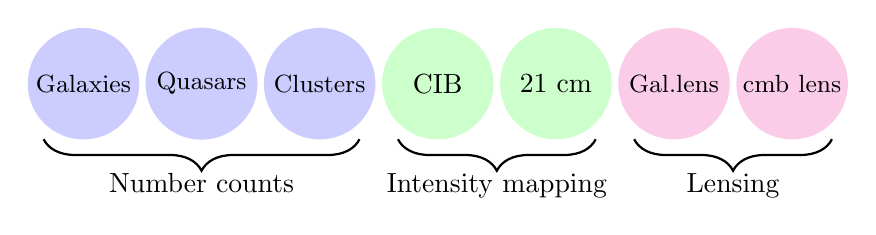
\begin{tikzpicture}[
			ball/.style={circle,align=center,inner sep=0,text width=1.4cm},
			ubrace/.style={decoration={brace,mirror,raise=2mm,amplitude=4mm},decorate}
		]
		\node[ball,fill=blue!20]    (A) at (0.0,0.0) {\small Galaxies};
		\node[ball,fill=blue!20]    (B) at (1.5,0.0) {\small Quasars};
		\node[ball,fill=blue!20]    (C) at (3.0,0.0) {\small Clusters};
		\node[ball,fill=green!20]   (D) at (4.5,0.0) {CIB};
		\node[ball,fill=green!20]   (E) at (6.0,0.0) {21 cm};
		\node[ball,fill=magenta!20] (F) at (7.5,0.0) {\small Gal.lens};
		\node[ball,fill=magenta!20] (G) at (9.0,0.0) {\small cmb lens};
		\draw[thick,ubrace] (A.south west) -- (C.south east) node[pos=0.5,anchor=north,yshift=-5mm] {Number counts};
		\draw[thick,ubrace] (D.south west) -- (E.south east) node[pos=0.5,anchor=north,yshift=-5mm] {Intensity mapping};
		\draw[thick,ubrace] (F.south west) -- (G.south east) node[pos=0.5,anchor=north,yshift=-5mm] {Lensing};
	\end{tikzpicture}
	\uncover<2->{Compared to these, CMB lensing is
	\begin{itemize}
		\item<3-> \color{green!50!black}Very clean (simple source, no astrophysics, linear regime)
		\item<4-> \color{green!50!black}Directly measures total (i.e. mostly dark) matter distribution
		\item<5-> \color{green!50!black}High redshift ($0.1\lesssim z\lesssim 10$)
		\item<6-> \color{red}Faint
		\item<7-> \color{red}Low resolution
		\item<8-> \color{red}No tomography
	\end{itemize}}
\end{frame}


\begin{frame}{How lensing distorts the CMB}
	\begin{center}
		\begin{tikzpicture}
			\only<1>{\node at (0,0) {\includegraphics[height=7cm]{lensing/T.png}};}%
			\only<2>{\node at (0,0) {\includegraphics[height=7cm]{lensing/T.png}};}%
			\only<3>{\node at (0,0) {\includegraphics[height=7cm]{lensing/TlT.png}};}%
			\only<4-5>{\node at (0,0) {\includegraphics[height=7cm]{lensing/TsT.png}};}%
			\only<2-4>{\node at (0,0) {\includegraphics[height=7cm]{lensing/phi_contours.png}};}%
		\end{tikzpicture}

		\only<1>{Unlensed\uncover<0>{p}}%
		\only<2>{Gravitational potential}%
		\only<3>{Lensed\uncover<0>{p}}%
		\only<4>{Lensed x10\uncover<0>{p}}%
		\only<5>{Non-Gaussian\uncover<0>{p}}%
	\end{center}
\end{frame}

\begin{frame}{How lensing distorts the CMB Polarization}
	\begin{center}
		\hspace*{-3mm}
		\begin{tabular}{cc}
			{\bf Q} ($\pm 20\mu$K) & {\bf U} ($\pm 20\mu$K) \\
			\only<1>{\includegraphics[height=5.5cm]{lensing/EBQ.png}}%
			\only<2>{\includegraphics[height=5.5cm]{lensing/EBlQ.png}}%
			&
			\only<1>{\includegraphics[height=5.5cm]{lensing/EBU.png}}%
			\only<2>{\includegraphics[height=5.5cm]{lensing/EBlU.png}}%
		\end{tabular}

		\only<1>{Unlensed}%
		\only<2>{Lensed}%
	\end{center}
\end{frame}

\begin{frame}{How lensing distorts E and B}
	\begin{center}
		\hspace*{-3mm}
		\begin{tabular}{cc}
			{\bf E} ($\pm 20\mu$K) & {\bf B} ($\pm 0.5\mu$K) \\
			\only<1>{\includegraphics[height=5.5cm]{lensing/E.png}}%
			\only<2>{\includegraphics[height=5.5cm]{lensing/EBlE.png}}%
			&
			\only<1>{\includegraphics[height=5.5cm]{lensing/B.png}}%
			\only<2>{\includegraphics[height=5.5cm]{lensing/EBlB.png}}%
		\end{tabular}

		\only<1>{Unlensed}%
		\only<2>{Lensed}%
	\end{center}
\end{frame}

\begin{frame}{Measuring CMB lensing}
	\begin{tikzpicture}
		\node at (-0.1, 3.8) {Which is lensed?};
		\node[text width=6cm] at (0,0) {
			\begin{tabular}{m{0.5cm}m{2.25cm}m{2.25cm}}
				T &
				\includegraphics[height=2.25cm]{maps/small_lensed_0.png} &
				\includegraphics[height=2.25cm]{maps/small_unlensed_0.png} \\
				\uncover<2->{E &
				\includegraphics[height=2.25cm]{maps/small_lensed_1.png} &
				\includegraphics[height=2.25cm]{maps/small_unlensed_1.png}} \\
				\uncover<7->{B &
				\includegraphics[height=2.25cm]{maps/small_lensed_2.png} &
				\includegraphics[height=2.25cm]{maps/small_unlensed_2.png}}
			\end{tabular}
		};
		\node[text width=6.8cm,anchor=north] at (5.5,4) {
			\begin{itemize}
				\item<3-> Must detect statistically
					\begin{center}
						\uncover<4->{%
						Without lensing \\
						$\ell_1$ \includegraphics[width=2.0cm]{lens_line_high.png}
						$\independent$
						\includegraphics[width=2.0cm]{lens_line_low.png} $\ell_2$}\\
						\uncover<5->{%
						Lensing distorts \\
						\includegraphics[width=4.0cm]{lens_line_orig.png} \\
						into \\
						\includegraphics[width=4.0cm]{lens_line_lensed.png} \\
						$\textrm{cov}(a_{\ell_1 m_1},a_{\ell_2,m_2}) \ne 0$}
					\end{center}
				\item<6-> Measure off-diagonal CMB covariance
				\item<8-> B-mode lensing has (almost) no cosmic variance
			\end{itemize}
		};
	\end{tikzpicture}
\end{frame}

\begin{frame}{Measurements}
	\centering
	\begin{itemize}
		\item<1-> ACT 2011: First detection of lensing power spectrum
		\item<2-> Planck 2015: $40\sigma$!
	\end{itemize}
	\begin{tikzpicture}
		\uncover<1>{\node at (0,0) {\includegraphics[height=6cm]{act_lens_spec11.pdf}};}
		\uncover<2>{\node at (0,0) {\includegraphics[height=6cm]{planck_spt_act_lensing.pdf}};}
	\end{tikzpicture}
\end{frame}

\begin{frame}{Stacked halo lensing}
	\centering
	\begin{tikzpicture}
		\only<1-3>{\node at (0,0) {
			\only<1>{\includegraphics[height=6.5cm]{actpol_halo_sim_nolens.png}}%
			\only<2>{\includegraphics[height=6.5cm]{actpol_halo_sim_lens.png}}%
			\only<3->{\includegraphics[height=6.5cm]{actpol_halo_sim_diff.png}}%
		};}
		\only<1-3>{\node at (0,3.8) {
			\only<1>{Unlensed}%
			\only<2>{Lensed}%
			\only<3->{Diff}%
		};}
	\end{tikzpicture} \\
	\footnotesize{Credit: Madhavacheril}
\end{frame}
\begin{frame}{ACTPol 2014: First detection @$3.2\sigma$}
	\centering
	\hspace*{-1.2cm}\begin{tikzpicture}
		\node at (0,0) {\includegraphics[height=5cm]{actpol_halo_stack.pdf}};
		\node at (6,0) {\includegraphics[height=5cm]{actpol_cluster_lens_spec_madhavacheril.png}};
	\end{tikzpicture}
	Madhavacheril et al. 2014, arXiv:1411.7999 \\
	Probes dark matter halo density profile
\end{frame}

%      - What it helps with ((geometric degeneracy), neutrino mass, bias, dark energy(how?))
%      - ACT results
%      - Planck dominates
% 35 * SZ
%      - tSZ, kSZ

\begin{frame}{Sunyaev Zel'dovich effect}
	\centering
	\begin{tikzpicture}
		\node at (0,0) {\includegraphics[height=6cm]{sz_illustration_van_speybroeck.png}};
		\uncover<2>{\node at (5.5,0) {\includegraphics[height=5cm]{sz_intensity_carlstrom.jpeg}};}
		\uncover<3-4>{\node at (5.5,-0.3) {\includegraphics[height=4.5cm]{sz_temperature.jpeg}};}
		\node at (0,-3.2) {\footnotesize{Credit: Van Speybroeck}};
		\uncover<2-4>{\node at (5.5,-3.1) {\footnotesize{Credit: Carlstrom}};};
		\uncover<4->{
			\node at (2.8,-4.0) {
				\includegraphics[height=1cm]{maps/sz1.png}
				\includegraphics[height=1cm]{maps/sz2.png}
				\includegraphics[height=1cm]{maps/sz3.png}
				\includegraphics[height=1cm]{maps/sz4.png}
				\includegraphics[height=1cm]{maps/sz5.png}
				\includegraphics[height=1cm]{maps/sz6.png}
				\includegraphics[height=1cm]{maps/sz7.png}
				\includegraphics[height=1cm]{maps/sz8.png}
				\includegraphics[height=1cm]{maps/sz9.png}
			};
			\node at (2.8,-4.6) {\footnotesize{Credit: Planck}};
		}
		\uncover<5>{
			\node[text width=5cm] at (5.5,0) {
				\begin{itemize}
					\item Distance independent: Detect massive clusters at any distance!
					\item Given pressure profile model: Measure mass and physical size of cluster
					\item Probe cluster mass distribution as function of redshift
				\end{itemize}
			};
		}
	\end{tikzpicture}
\end{frame}
\begin{frame}{ACT Measurements}
	\includegraphics[width=\textwidth]{act_sz_clusters.eps} \\
	\begin{tikzpicture}
		\node[text width=5cm] at (0,0.5) {
			\begin{itemize}
				\item ACT detected 68 clusters
				\item Cosmology limited by pressure profile
				\item ACTPol analysis ongoing
			\end{itemize}
		};
		\node at (5,0) {\includegraphics[width=4cm]{act_sz_cosmology.eps}};

	\end{tikzpicture}

\end{frame}

\begin{frame}{Kinematic SZ}
	\begin{tikzpicture}
		\node at (0,0) {\includegraphics[height=6cm]{sz_illustration_van_speybroeck.png}};
		\node at (5.5,-0.3) {\includegraphics[height=4.5cm]{sz_temperature.jpeg}};
		\node at (0,-3.2) {\footnotesize{Credit: Van Speybroeck}};
		\node at (5.5,-3.1) {\footnotesize{Credit: Carlstrom}};
		\uncover<2->{
		\draw [thick,red,->] (-1.7,-0.0) -- +(0,-0.5);
		\draw [thick,red,->] (-1.3,-0.35) -- +(0,-0.5);
		\draw [thick,red,->] (-0.9,-0.45) -- +(0,-0.5);
		\draw [thick,red,->] (-0.5,-0.50) -- +(0,-0.5);
		\draw [thick,red,->] ( 0.5,-0.40) -- +(0,-0.5);
		\draw [thick,red,->] ( 0.9,-0.30) -- +(0,-0.5);
		\draw [thick,red,->] ( 1.3, 0.30) -- +(0,-0.5);}
		\uncover<3->{
			\draw [thick,red] (3.94,1.089) -- +(0.25,0.0) -- +(0.50,0.01) -- +(0.75,0.022) -- +(1.00,0.035) -- +(1.5,0.067)-- +(2.0,0.090) -- +(2.5,0.098) -- +(3.88,0.110);
		}
	\end{tikzpicture}
\end{frame}

\begin{frame}{Kinematic SZ}
	\begin{tikzpicture}
		\node at (0,0) {\includegraphics[height=8cm]{sz_act_boss_sudeep.jpeg}};
		\node at (5.5,-2) {\includegraphics[width=6cm]{actpol_ksz_detection.png}};
		\node[text width=7cm] at (5.5,2) {
			\begin{itemize}
				\item Very faint ($\sim 20$ times weaker than kSZ)
				\item Hard to distinguish from CMB + tSZ
				\item First detection by ACT in 2012 via pairwise comparison of 5000 galaxies

			\end{itemize}
		};
	\end{tikzpicture}
\end{frame}
%      - first detection of kSZ?
% 40 * Summary of ACT firsts
%    * Future: Full ACTPol and Advanced act
\begin{frame}
	\centering
	\hspace*{-0.8cm}\includegraphics[width=12.5cm]{advact_sky_coverage.png} \\
	\includegraphics[width=\textwidth]{advact_multichroic.png}
\end{frame}
\begin{frame}
	\centering
	\hspace*{-1cm}\begin{tikzpicture}
		\node at (0, 2) {\includegraphics[height=5.2cm]{advact_polspec_forecast.png}};
		\node at (0.3,-2.1) {\includegraphics[height=3cm,width=5cm]{advact_lensing_forecast_blake.png}};
		\node at (0.5, -1) {\small CMB lensing};
		\node[red] at (0.3,-2.5) {$\sim220\sigma$};
		\node at (0.3,-3.2) {\footnotesize{Credit: Blake Sherwin}};
		\node at (5, 2) {\includegraphics[width=4.3cm]{advact_cluster_forecast.pdf}};
		\node at (5,-2.05) {\includegraphics[width=4cm]{advact_dsfg_forecast.pdf}};
	\end{tikzpicture}
\end{frame}
% 45 * End
\begin{frame}{Summary}
	\begin{itemize}
		\item ACT is one of two high-resolution CMB experiments
		\item High resolution reveals blemishes and distortions
		\item These are relatively clean probes of the rest of the universe
		\item First analysis of 2013 data complete; currently working on 2014 data
		\item Advanced ACT set to start in 2016
	\end{itemize}
\end{frame}

% Pretty long!

\begin{frame}{Bonus slides}
\end{frame}

\begin{frame}{Map noise properties}
	\centering
	\includegraphics[width=0.7\textwidth]{maps/noise_sim.png}
\end{frame}
\begin{frame}{CMB sim for comparison}
	\centering
	\includegraphics[width=0.7\textwidth]{maps/cmb_sim.png}
\end{frame}

\begin{frame}
	\centering
	\begin{tabular}{c}
		\only<1>{Total signal}%
		\only<2>{CMB (Wiener)}%
		\only<3>{Remainder}%
		\only<4>{Total signal}%
		\\
		\only<1>{\includegraphics[width=0.7\textwidth]{maps/crop/coadd.png}}%
		\only<2>{\includegraphics[width=0.7\textwidth]{maps/crop/cmb.png}}%
		\only<3>{\includegraphics[width=0.7\textwidth]{maps/crop/nocmb.png}}%
		\only<4>{\includegraphics[width=0.7\textwidth]{maps/crop/coadd.png}}%
		\\
		$\pm 250 \mu$K, $4.26^\circ \times 4.26^\circ$
	\end{tabular}
\end{frame}

\begin{frame}{E,B and Q, U}
	\begin{center}
		\only<1>{E and B result from quadrupole-convolutions of Q and U}%
		\only<2>{Reverse also holds}%

	\scalebox{1.7}{
		\begin{minipage}{5cm}
			\begin{align*}
				\only<1>{%
				E =& \rmimg{contaminants/queb_0.png}{1cm} \otimes Q + \mimg{contaminants/queb_2.png}{1cm} \otimes U \\
				B =& \mimg{contaminants/queb_1.png}{1cm} \otimes Q + \rmimg{contaminants/queb_3.png}{1cm} \otimes U}%
				\only<2>{%
				Q =& \rmimg{contaminants/ebqu_0.png}{1cm} \otimes E + \mimg{contaminants/ebqu_2.png}{1cm} \otimes B \\
				U =& \mimg{contaminants/ebqu_1.png}{1cm} \otimes E + \rmimg{contaminants/ebqu_3.png}{1cm} \otimes B}%
			\end{align*}
		\end{minipage}}
	\end{center}
\end{frame}

\begin{frame}{E, B and Q, U}
	\begin{center}
		\includegraphics[height=8cm]{EB_healpix.pdf}
	\end{center}
\end{frame}

\end{document}
